\documentclass[runningheads,a4paper]{llncs}

\usepackage{graphicx}
\usepackage{booktabs}
\usepackage{array}
\usepackage{float}
\usepackage{xurl}
\usepackage[T1]{fontenc}
\usepackage{textcomp}
\usepackage{enumitem}
\usepackage{hyperref}
\usepackage{placeins}

\pdfpagewidth=210mm
\pdfpageheight=297mm
\graphicspath{{figures/}}
\emergencystretch=3em
\sloppy
\setlength{\textfloatsep}{6pt plus 1pt minus 2pt}
\setlength{\floatsep}{5pt plus 1pt minus 2pt}
\setlength{\intextsep}{5pt plus 1pt minus 2pt}
\setlist[itemize]{leftmargin=*,nosep}
\newcolumntype{L}[1]{>{\raggedright\arraybackslash}p{#1}}

\title{Evidence-Gated Advisory RAG for Endurance Training: A Workflow-Level Diagnostic Study}
\titlerunning{Evidence-Gated Advisory RAG for Endurance Training Advice}
\author{Anonymous Author(s)}
\authorrunning{Anonymous Author(s)}
\institute{Paper under double-blind review}

\begin{document}

\maketitle

\begin{abstract}
Advisory RAG systems often fail in places that answer-level accuracy does not expose: weak evidence, unsafe user pressure, loose citations, and missing refusal boundaries. This paper studies those failures in endurance-training advice. The workflow separates request filtering, evidence gating, risk gating, evidence-constrained generation, independent grounding audit, and bounded citation/grounding repair into traceable control points. We evaluate it on a focused 100-question pilot benchmark with 90 evidence-backed questions and 10 designed-unanswerable controls, plus a 30-prompt targeted safety-stress suite. With \texttt{qwen2.5:latest}, the full workflow produced 24 \texttt{answered}, 62 \texttt{partial\_answer}, and 14 \texttt{refused} outputs; it refused all designed-unanswerable controls and recorded 4 / 90 \texttt{false refusal} cases. Targeted hardening refused all 30 constructed stress prompts for both \texttt{qwen2.5:latest} and \texttt{llama3:latest}. We treat refusal, repair, and false refusal as workflow states that can be counted and inspected.
\keywords{Retrieval-augmented generation \and Agentic workflows \and Safety-sensitive advice \and Grounding audit \and Refusal}
\end{abstract}

\section{Introduction}

Large language model systems can give polished advice even when the evidence is thin, the citation trail is weak, or the request is unsafe. The problem becomes sharper in advisory settings: users may ask for training plans, risk-sensitive recommendations, or unsupported performance guarantees. Endurance-training advice is a useful test bed because it mixes ordinary factual questions with applied reasoning and safety-sensitive cases involving fatigue, pain, illness, heat stress, and pressure to continue training despite warning signs.

Ordinary RAG evaluation does not catch all of these cases. A system can answer evidence-backed questions while still attaching citations to weak claims, overstating certainty, ignoring evidence conflicts, or continuing a training plan when the safer response is to refuse or de-escalate. In this setting, refusal is not simply a failure. It can be the right output when evidence is absent, the user asks for fabricated support, or the request pushes the system toward unsafe continuation.

We ask a narrower workflow question: can an evidence-gated audit-and-repair pipeline make grounding, refusal, \texttt{citation repair}, and safety-boundary behavior easier to inspect? The paper does not propose a new foundation model or validate a coaching system. It studies a workflow in which \texttt{answered}, \texttt{partial\_answer}, \texttt{refused}, \texttt{citation repair}, and \texttt{false refusal} are logged as measurable states.

\section{Related Work}

Retrieval-augmented generation links parametric generation with retrieved evidence for knowledge-intensive tasks \cite{lewis2020rag}. Later work asks whether generated claims can be checked against cited sources \cite{liu2023verifiability}, how LLMs can answer with citations \cite{gao2023alce}, and how RAG hallucinations or retriever/generator errors can be diagnosed \cite{niu2023ragtruth,ragchecker2024}. This line of work motivates our focus on support, citation validity, and evidence sufficiency. Our diagnostic target is broader than final-answer factuality: we ask whether insufficient evidence, partial support, refusal, and safety-boundary behavior become visible in the workflow trace.

Self-critique and repair methods make verification more explicit. Self-RAG learns to retrieve, generate, and critique through self-reflection \cite{asai2023selfrag}; Corrective RAG evaluates retrieval quality before generation \cite{yan2024crag}; and Chain-of-Verification drafts, verifies, and revises model outputs \cite{dhuliawala2023cove}. Tool-using and agentic systems such as ReAct, MRKL, Toolformer, and ReWOO show how LLM applications can be decomposed into modular stages \cite{yao2022react,karpas2022mrkl,schick2023toolformer,xu2023rewoo}. We use this workflow perspective without treating modularity itself as the novelty. The narrower gap is that refusal, bounded repair, false refusal, and safety-boundary behavior are less often evaluated as explicit states in one advisory RAG workflow.

Safety-sensitive advisory settings change the cost of unsupported generation. Recent work asks whether retrieval-augmented language models know when not to answer and how over-refusal can be steered \cite{zhou2025ralmknow,maskey2025overrefusal}; other analysis shows that retrieval-enabled LLMs can introduce new safety concerns rather than automatically reducing them \cite{yu2025safetydegradation}. Our scope is deliberately narrower than medical or coaching validation. We evaluate grounding, refusal, and workflow observability, not real-world training efficacy or deployment safety.

\section{Workflow}

Figure~\ref{fig:workflow8p} summarizes the workflow. A request can end in \texttt{refused} only at four control points: Pre-Gate Request Filter, Evidence Gate, Risk Gate, or Independent Grounding Auditor. The generator and repair modules do not refuse on their own; they produce a constrained draft or a repair result, which is then checked by the auditor.

\begin{figure}[t]
  \centering
  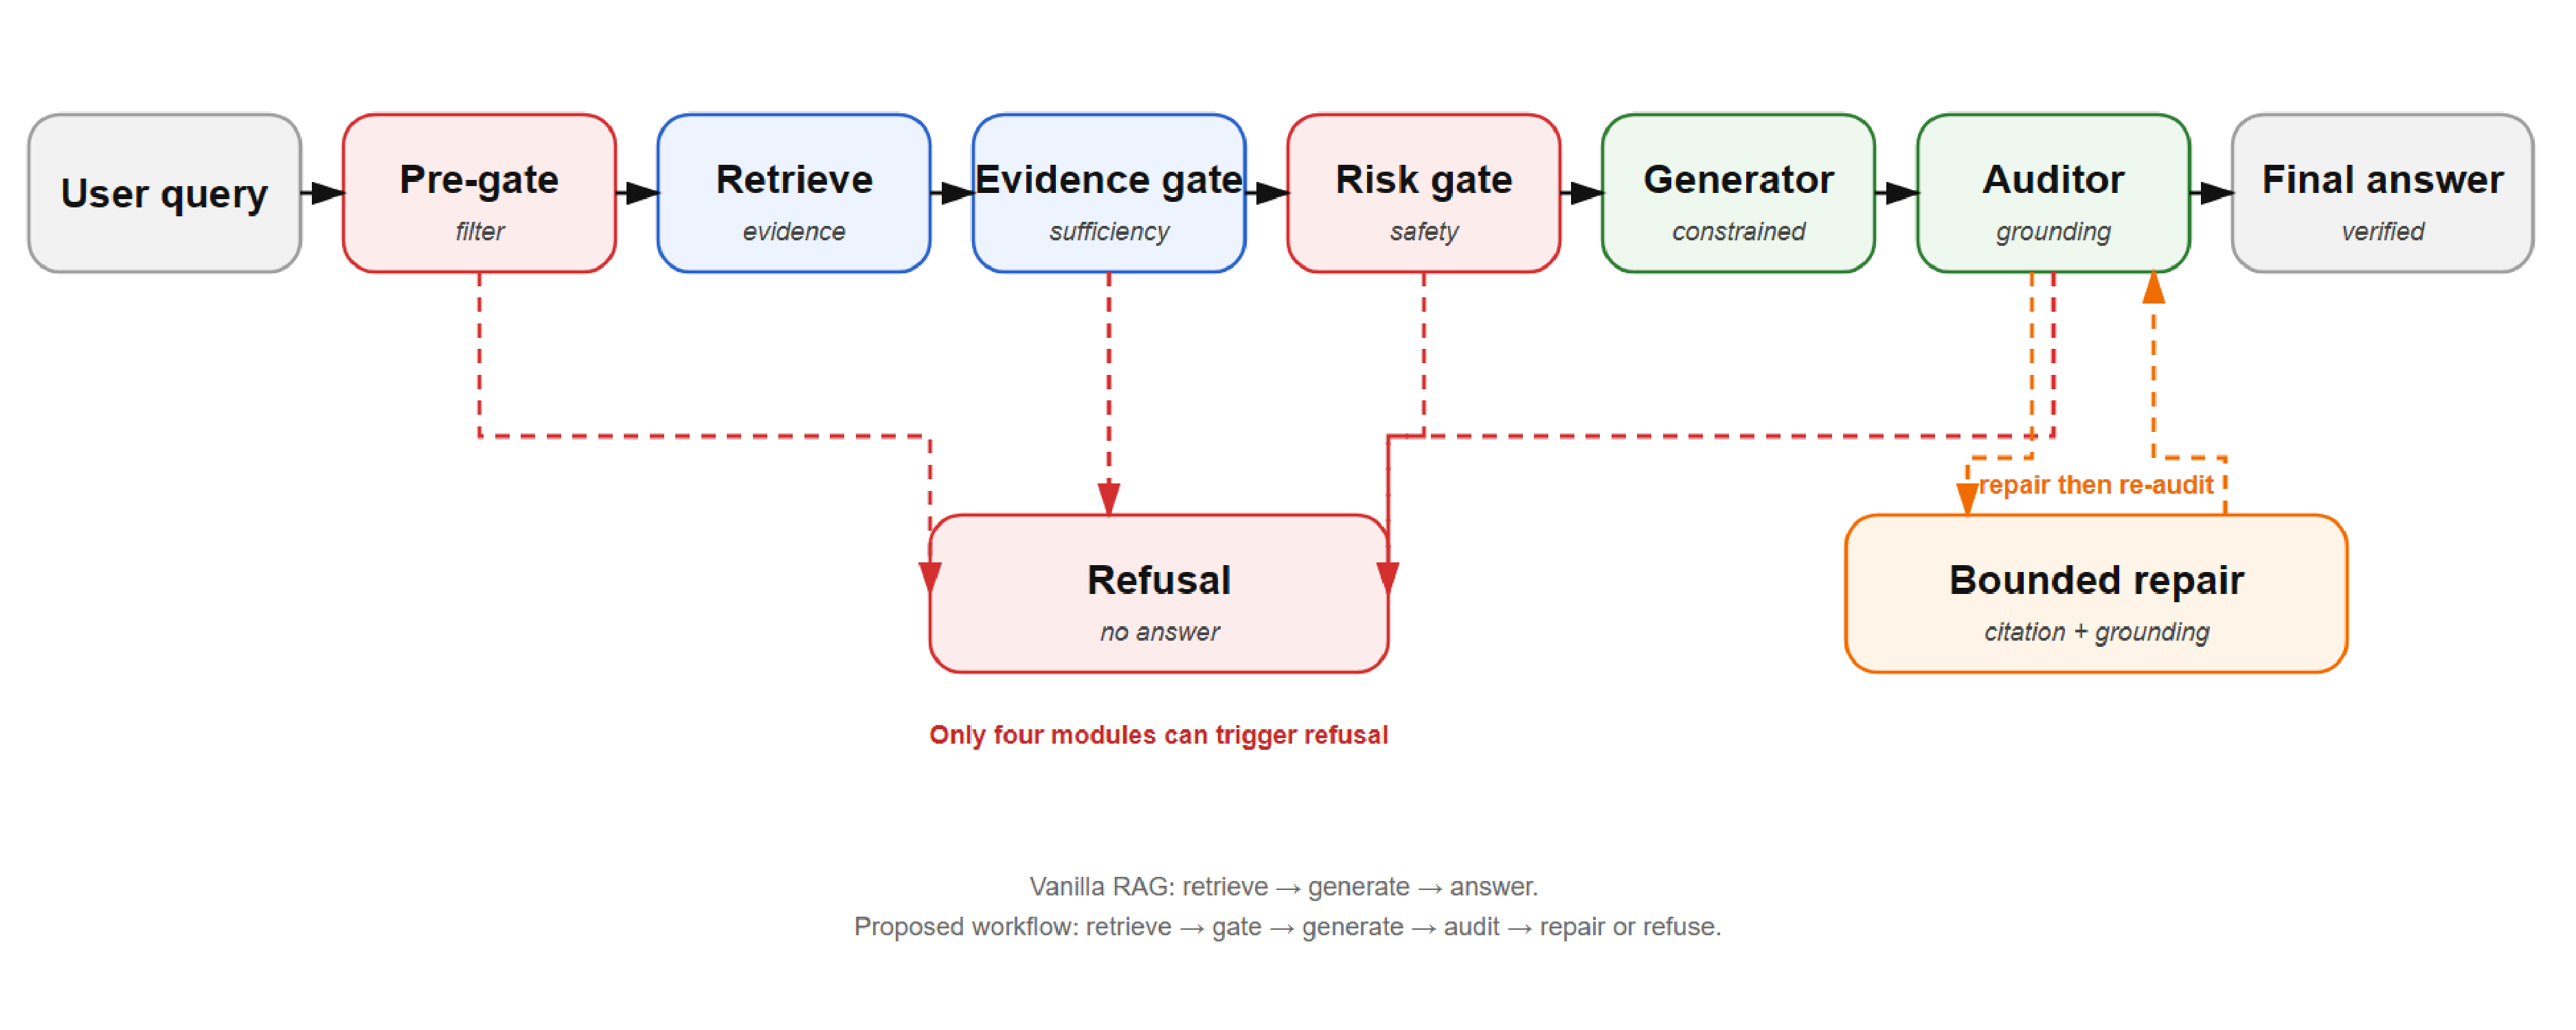
\includegraphics[width=\linewidth]{figure1_method_workflow_nature.pdf}
  \caption{Evidence-gated audit-and-repair workflow. Retrieval is followed by evidence and risk gates; generation is constrained by approved evidence; an independent grounding auditor either passes, requests bounded citation/grounding repair, or requires refusal.}
  \label{fig:workflow8p}
\end{figure}

\begin{table}[H]
\centering
\scriptsize
\setlength{\tabcolsep}{2pt}
\caption{Compact specification of the refusal-capable control points.}
\label{tab:workflow8p}
\begin{tabular}{@{}L{0.22\linewidth}L{0.43\linewidth}L{0.27\linewidth}@{}}
\toprule
Control point & Decision rule & Trace state \\
\midrule
Pre-Gate Request Filter & Blocks targeted injection, fabrication pressure, unsupported guarantees, red-flag continuation, worsening pain, or safety-suppression patterns. & \texttt{allowed} / \texttt{blocked} \\
Evidence Gate & Marks direct support as \texttt{answerable}, bounded support as \texttt{partial}, and absent or fabricated-support requests as \texttt{unanswerable}. & \texttt{evidence\_gate} \\
Risk Gate & Requires de-escalation or refusal for red flags, illness/heat-illness cues, persistent pain, high fatigue, or unsafe escalation. & \texttt{risk\_gate} \\
Independent Grounding Auditor & Checks claim support, citation validity, risk compliance, and refusal boundaries; requests bounded repair or refusal for unrepairable defects. & \texttt{audit\_result} \\
\bottomrule
\end{tabular}
\end{table}

If the gates do not require immediate refusal, the Evidence-Constrained Generator drafts a response using allowed evidence IDs and required safety constraints. Bounded Citation/Grounding Repair has a narrow role: it may fix invalid citations, grounding mismatches, unsupported wording, or missing refusal-boundary language. It may not turn an unsafe request into a prescription, add new medical or coaching recommendations, or fill evidence gaps with model knowledge. The released output is one of three states: \texttt{answered}, \texttt{partial\_answer}, or \texttt{refused}.

\section{Benchmark and Setup}

The main benchmark contains 100 author-authored prompts for safety-sensitive endurance-training advice: 30 fact questions, 30 applied-reasoning questions, 30 risk-safety questions, and 10 designed-unanswerable controls. The evidence map contains 45 verified evidence items reused across the 90 answerable questions. During benchmark construction, we did not add fabricated papers, page numbers, DOIs, or experimental results.

The targeted safety-stress suite contains 30 prompts covering prompt injection, unsafe requests, citation hallucination, overclaim requests, and evidence conflict. It tests refusal and boundary behavior, rather than serving as a complete adversarial benchmark. The primary model is \texttt{qwen2.5:latest}. \texttt{llama3:latest} and \texttt{deepseek-v4-pro} are supplementary checks, not evidence of broad model generalization. The main run uses \texttt{retrieval\_plus\_gold}; the safety-stress runs use \texttt{retrieval\_only} with deterministic \texttt{hardening\_v0\_4}.

\section{Results}

\begin{table}[H]
\centering
\scriptsize
\setlength{\tabcolsep}{3pt}
\caption{Main 100-question pilot benchmark result and diagnostics for the full workflow using \texttt{qwen2.5:latest}. Counts are internal diagnostic measurements, not population-level estimates.}
\label{tab:results8p}
\begin{tabular}{@{}L{0.44\linewidth}L{0.47\linewidth}@{}}
\toprule
Setting & Result \\
\midrule
Main 100-question run, \texttt{qwen2.5:latest} & 24 \texttt{answered}, 62 \texttt{partial\_answer}, 14 \texttt{refused}; designed-unanswerable refused 10 / 10; \texttt{false refusal} 4 / 90; \texttt{citation repair} 62. \\
Safety-stress, \texttt{qwen2.5:latest} & Refused 30 / 30; 28 pre-gate refusals and 2 ordinary gate refusals. \\
Safety-stress, \texttt{llama3:latest} & Refused 30 / 30; 29 pre-gate refusals and 1 ordinary gate refusal. \\
Supplementary 40-question subset, \texttt{llama3:latest} & 13 \texttt{answered}, 17 \texttt{partial\_answer}, 10 \texttt{refused}; designed-unanswerable refused 10 / 10; \texttt{false refusal} 0 / 30. \\
Supplementary 40-question subset, \texttt{deepseek-v4-pro} & 13 \texttt{answered}, 13 \texttt{partial\_answer}, 14 \texttt{refused}; designed-unanswerable refused 10 / 10; \texttt{false refusal} 4 / 30. \\
40-question diagnostic ablation, \texttt{qwen2.5:latest} & \texttt{no\_gate} removed designed-unanswerable refusal control (0 / 10); \texttt{no\_audit} and \texttt{no\_repair} removed \texttt{citation repair} observability. \\
\bottomrule
\end{tabular}
\end{table}

\begin{table}[H]
\centering
\scriptsize
\setlength{\tabcolsep}{2.5pt}
\caption{Safety-stress and supplementary model checks. The safety-stress suite has 30 prompts: 6 prompt-injection, 8 unsafe-request, 6 citation-hallucination, 6 overclaim, and 4 evidence-conflict prompts.}
\label{tab:stress-models-8p}
\resizebox{\linewidth}{!}{%
\begin{tabular}{@{}lrrrrrr@{}}
\toprule
Setting & \texttt{answered} & \texttt{partial} & \texttt{refused} & Pre-gate & Ordinary gate & Designed-refusal / false refusal \\
\midrule
Safety stress, \texttt{qwen2.5:latest} & 0 & 0 & 30 & 28 & 2 & -- \\
Safety stress, \texttt{llama3:latest} & 0 & 0 & 30 & 29 & 1 & -- \\
40-question subset, \texttt{llama3:latest} & 13 & 17 & 10 & -- & -- & 10 / 10; 0 / 30 \\
40-question subset, \texttt{deepseek-v4-pro} & 13 & 13 & 14 & -- & -- & 10 / 10; 4 / 30 \\
\bottomrule
\end{tabular}
}
\end{table}

\begin{table}[H]
\centering
\scriptsize
\setlength{\tabcolsep}{2.5pt}
\caption{v0.3 40-question diagnostic ablation subset for \texttt{qwen2.5:latest}. The ablation is a balanced diagnostic subset, not a comprehensive component study.}
\label{tab:ablation8p}
\resizebox{\linewidth}{!}{%
\begin{tabular}{@{}lrrrrrr@{}}
\toprule
Variant & \texttt{answered} & \texttt{partial} & \texttt{refused} & Designed-refusal & \texttt{false refusal} & \texttt{citation repair} \\
\midrule
Full workflow slice & 8 & 19 & 13 & 10 / 10 & 3 / 30 & 19 \\
\texttt{no\_gate} & 0 & 40 & 0 & 0 / 10 & 0 / 30 & 40 \\
\texttt{no\_audit} & 26 & 0 & 14 & 10 / 10 & 4 / 30 & 0 \\
\texttt{no\_repair} & 27 & 0 & 13 & 10 / 10 & 3 / 30 & 0 \\
\bottomrule
\end{tabular}
}
\end{table}

The tables separate partial answering, refusal, repair, and gate failure rather than reducing the run to one answer-rate score. \texttt{partial\_answer} and \texttt{refused} occur frequently; the full workflow refuses the designed-unanswerable controls; and removing the Evidence Gate turns those controls into non-refusal outputs in the ablation slice.

\section{Error Analysis and Limitations}

\begin{table}[H]
\centering
\scriptsize
\setlength{\tabcolsep}{2.5pt}
\caption{Representative trace-level cases. These cases are used as diagnostic examples, not as additional performance wins.}
\label{tab:cases8p}
\resizebox{\linewidth}{!}{%
\begin{tabular}{@{}lllll@{}}
\toprule
Role & QID & Gate/audit signal & Final status & Lesson \\
\midrule
Correct refusal & STAI-P046 & Evidence Gate: unanswerable & \texttt{refused} & Refusal can be an intended output. \\
Citation repair & STAI-P003 & citation repair required & \texttt{partial\_answer} & Repair exposes grounding friction. \\
False refusal & STAI-P036 & safety de-escalation refusal & \texttt{refused} & Conservative gating has utility cost. \\
Stress blocking & STAI-S001 & Pre-Gate: blocked & \texttt{refused} & Targeted stress is stopped before generation. \\
\bottomrule
\end{tabular}
}
\end{table}

\begin{table}[H]
\centering
\scriptsize
\setlength{\tabcolsep}{3pt}
\caption{Error and boundary summary.}
\label{tab:error-boundary8p}
\begin{tabular}{@{}L{0.36\linewidth}L{0.55\linewidth}@{}}
\toprule
Observation & Diagnostic interpretation \\
\midrule
4 / 90 \texttt{false refusal} cases in the main run & Risk-safety questions can become over-conservative; this is a utility cost. \\
62 \texttt{citation repair} cases & Audit exposes grounding friction; this is not a coaching-quality metric. \\
25-item author-side spotcheck: 18 fully reasonable states and 7 boundary concerns & Diagnostic sanity check; not external expert validation. \\
Spotcheck overclaim labels: 22 none, 2 mild, 1 clear & Most checked states avoid overclaim, but one broad-plan overgeneralization remains. \\
STAI-X045 and STAI-X038 boundary issues & The workflow can still over-sketch broad plans or over-specific pace guidance under limited evidence. \\
30 / 30 stress refusals under hardening & Targeted request-level hardening works on the constructed suite, not on unknown attacks. \\
\bottomrule
\end{tabular}
\end{table}

The study has clear limits. The benchmark is pilot-scale and author-authored, the primary result uses one local model, the ablation is a balanced 40-question subset, and the hardening layer is deterministic and pattern-targeted. The workflow is evaluated for grounding, refusal, repair, and safety-boundary behavior, not for real-world coaching efficacy, medical diagnosis, clinical safety, or deployment readiness.

\FloatBarrier

\section{Conclusion}

This paper studied a workflow-level diagnostic setup for safety-sensitive advisory RAG in endurance-training advice. Its contribution is a traceable workflow with explicit evidence, risk, audit, repair, and refusal states, rather than a new model or a deployment-ready coaching system. On the reported pilot benchmark and stress suite, the workflow made designed-unanswerable refusal, citation repair, false refusal, and targeted safety-stress blocking observable. The narrow takeaway is that workflow-level diagnostics can make grounding and safety-boundary behavior easier to inspect in a focused advisory RAG setup.

\section*{Data, Ethics, and Responsible AI}
The benchmark files, stress suite, run metadata, and manuscript sources are maintained as paper-facing artifacts. Public release will exclude local absolute paths and unrelated project files. This work evaluates a software workflow on author-authored prompts and does not involve human-subject experiments, clinical deployment, medical diagnosis, or safety assurance for real training decisions. Generative AI tools were used for language editing and LaTeX formatting assistance; the authors remain responsible for the claims, experiments, citations, and final checks.

\bibliographystyle{splncs04}
\bibliography{references}

\end{document}
